\documentclass[12pt]{beamer}
\usetheme{Madrid}
\usepackage[utf8]{inputenc}
\usepackage[spanish]{babel}
\usepackage{amsmath}
\usepackage{amsfonts}
\usepackage{amssymb}
\usepackage{multicol}
\usepackage{graphicx}
\graphicspath{ {./images/} }

\author[Edgar, Shah, Ronald]{Edgar Luque \and Shah Sawar \and Ronald Intriago}
\title{Gymodo}
\subtitle{La mejor app para tu gym} 


\definecolor{gymodo_orange}{rgb}{1, 0.556, 0.235}

\definecolor{UBCblue}{rgb}{0.04706, 0.13725, 0.26667}
\usecolortheme[named=UBCblue]{structure}

%\setbeamercovered{transparent} 
%\setbeamertemplate{navigation symbols}{} 
\logo{
\includegraphics[height=1cm]{gymodo_logo}} 
\institute[2WIAM]{
Proyecto de Desarrollo de Aplicaciones Multiplataforma \\
2WIAM \\
Escola del Treball de Barcelona
} 
\date[17-05-2021]{17 de mayo de 2021} 

\begin{document}

\begin{frame}
\titlepage
\end{frame}

\begin{frame}
\tableofcontents
\end{frame}

\begin{frame}{Visualización de la app}

\begin{columns}[t]
\column{.25\textwidth}
\centering
\includegraphics[width=\textwidth]{gymodo_home}
\column{.25\textwidth}
\centering
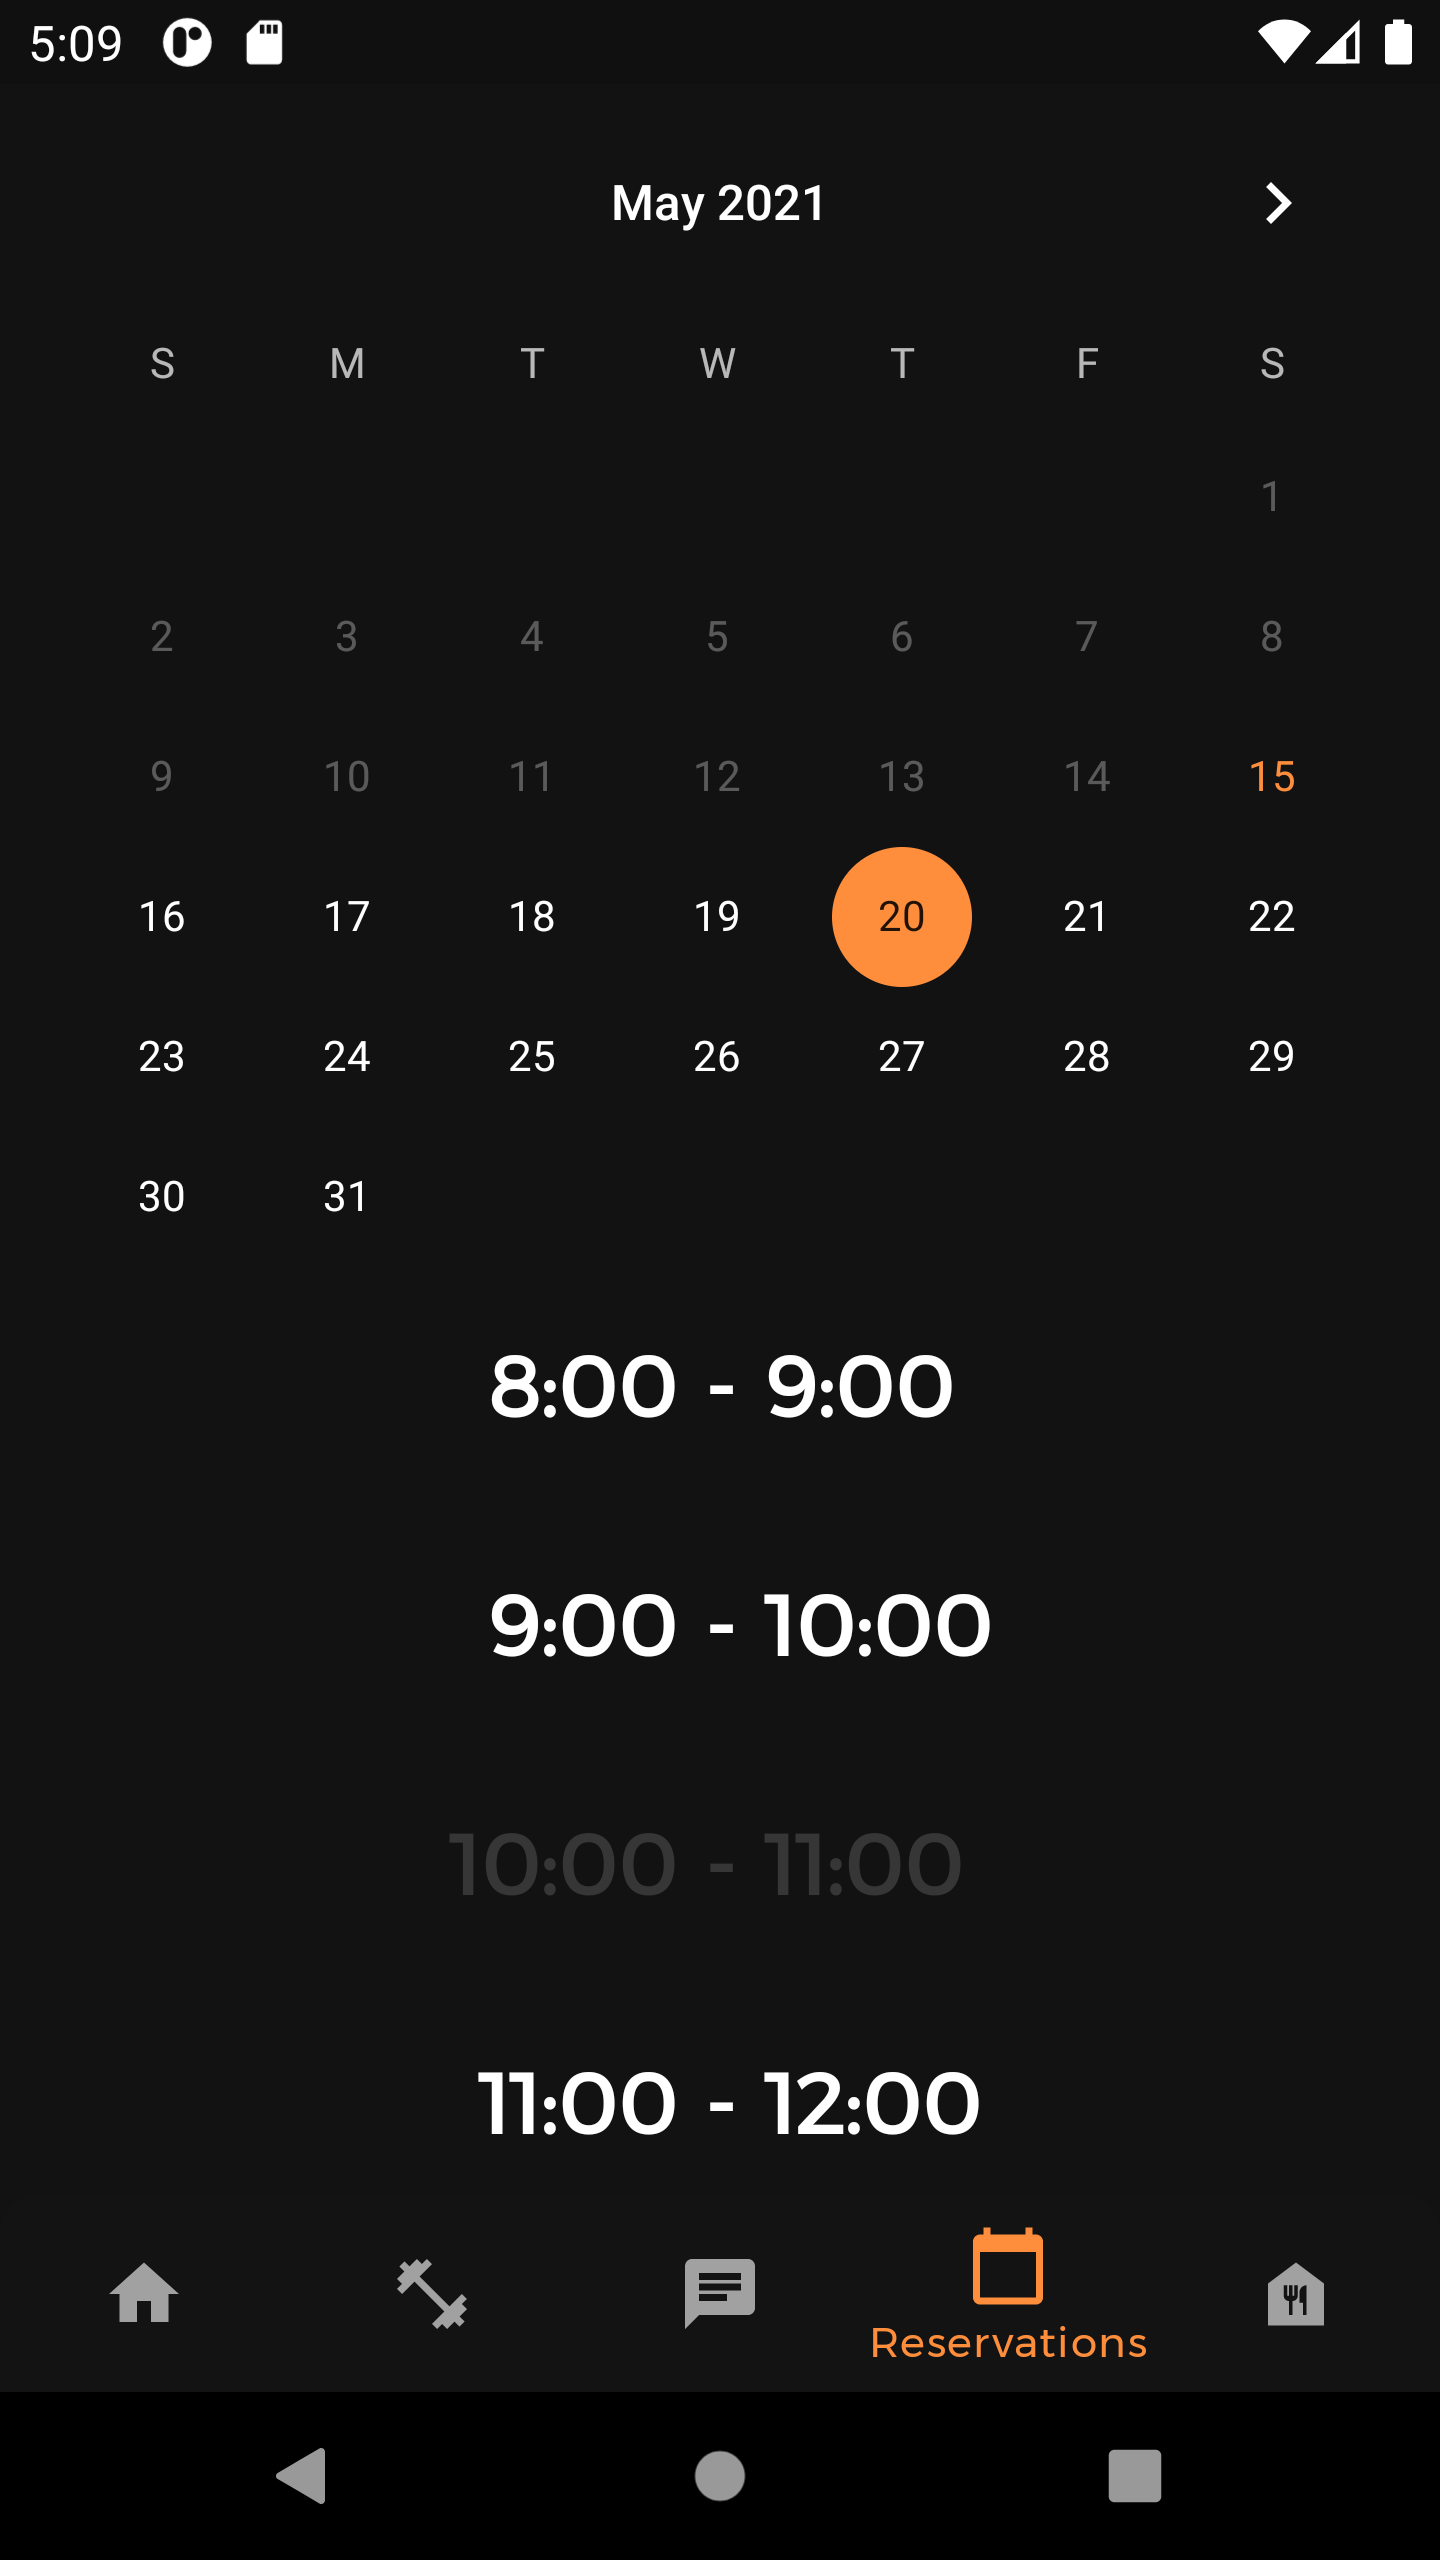
\includegraphics[width=\textwidth]{gymodo_create_reservation}
\column{.25\textwidth}
\centering
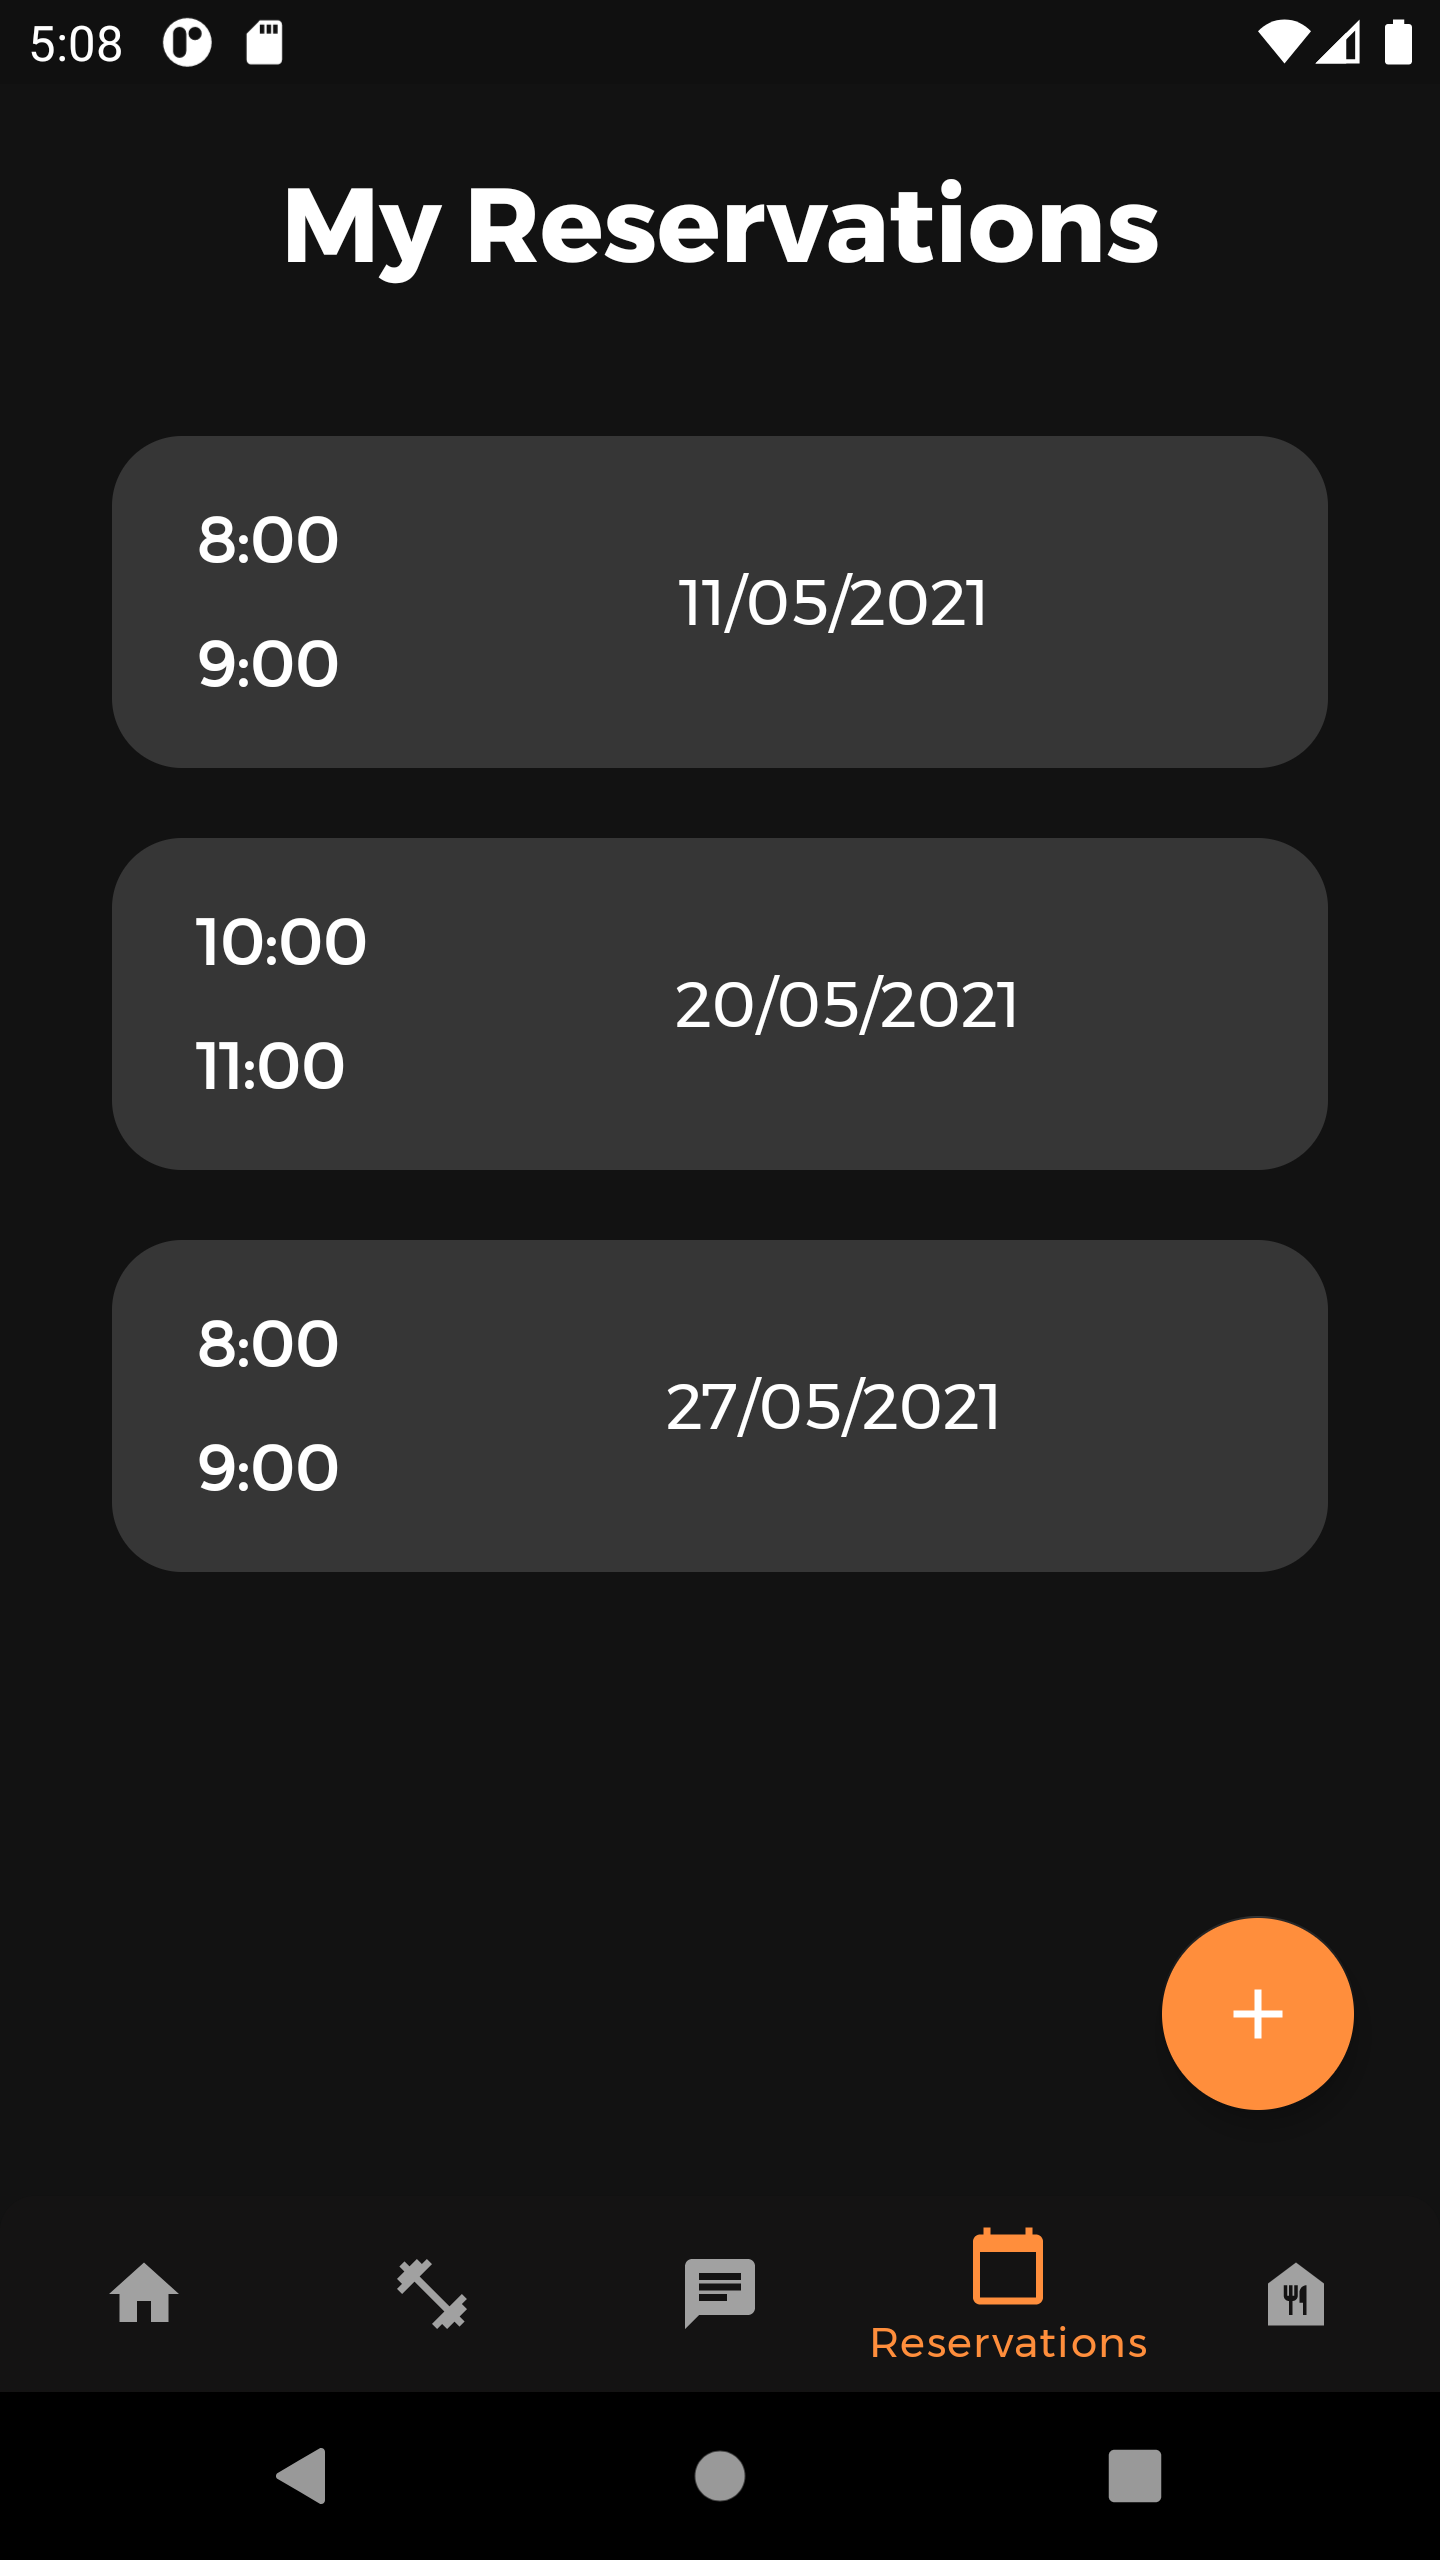
\includegraphics[width=\textwidth]{gymodo_your_reservations}
\column{.25\textwidth}
\centering
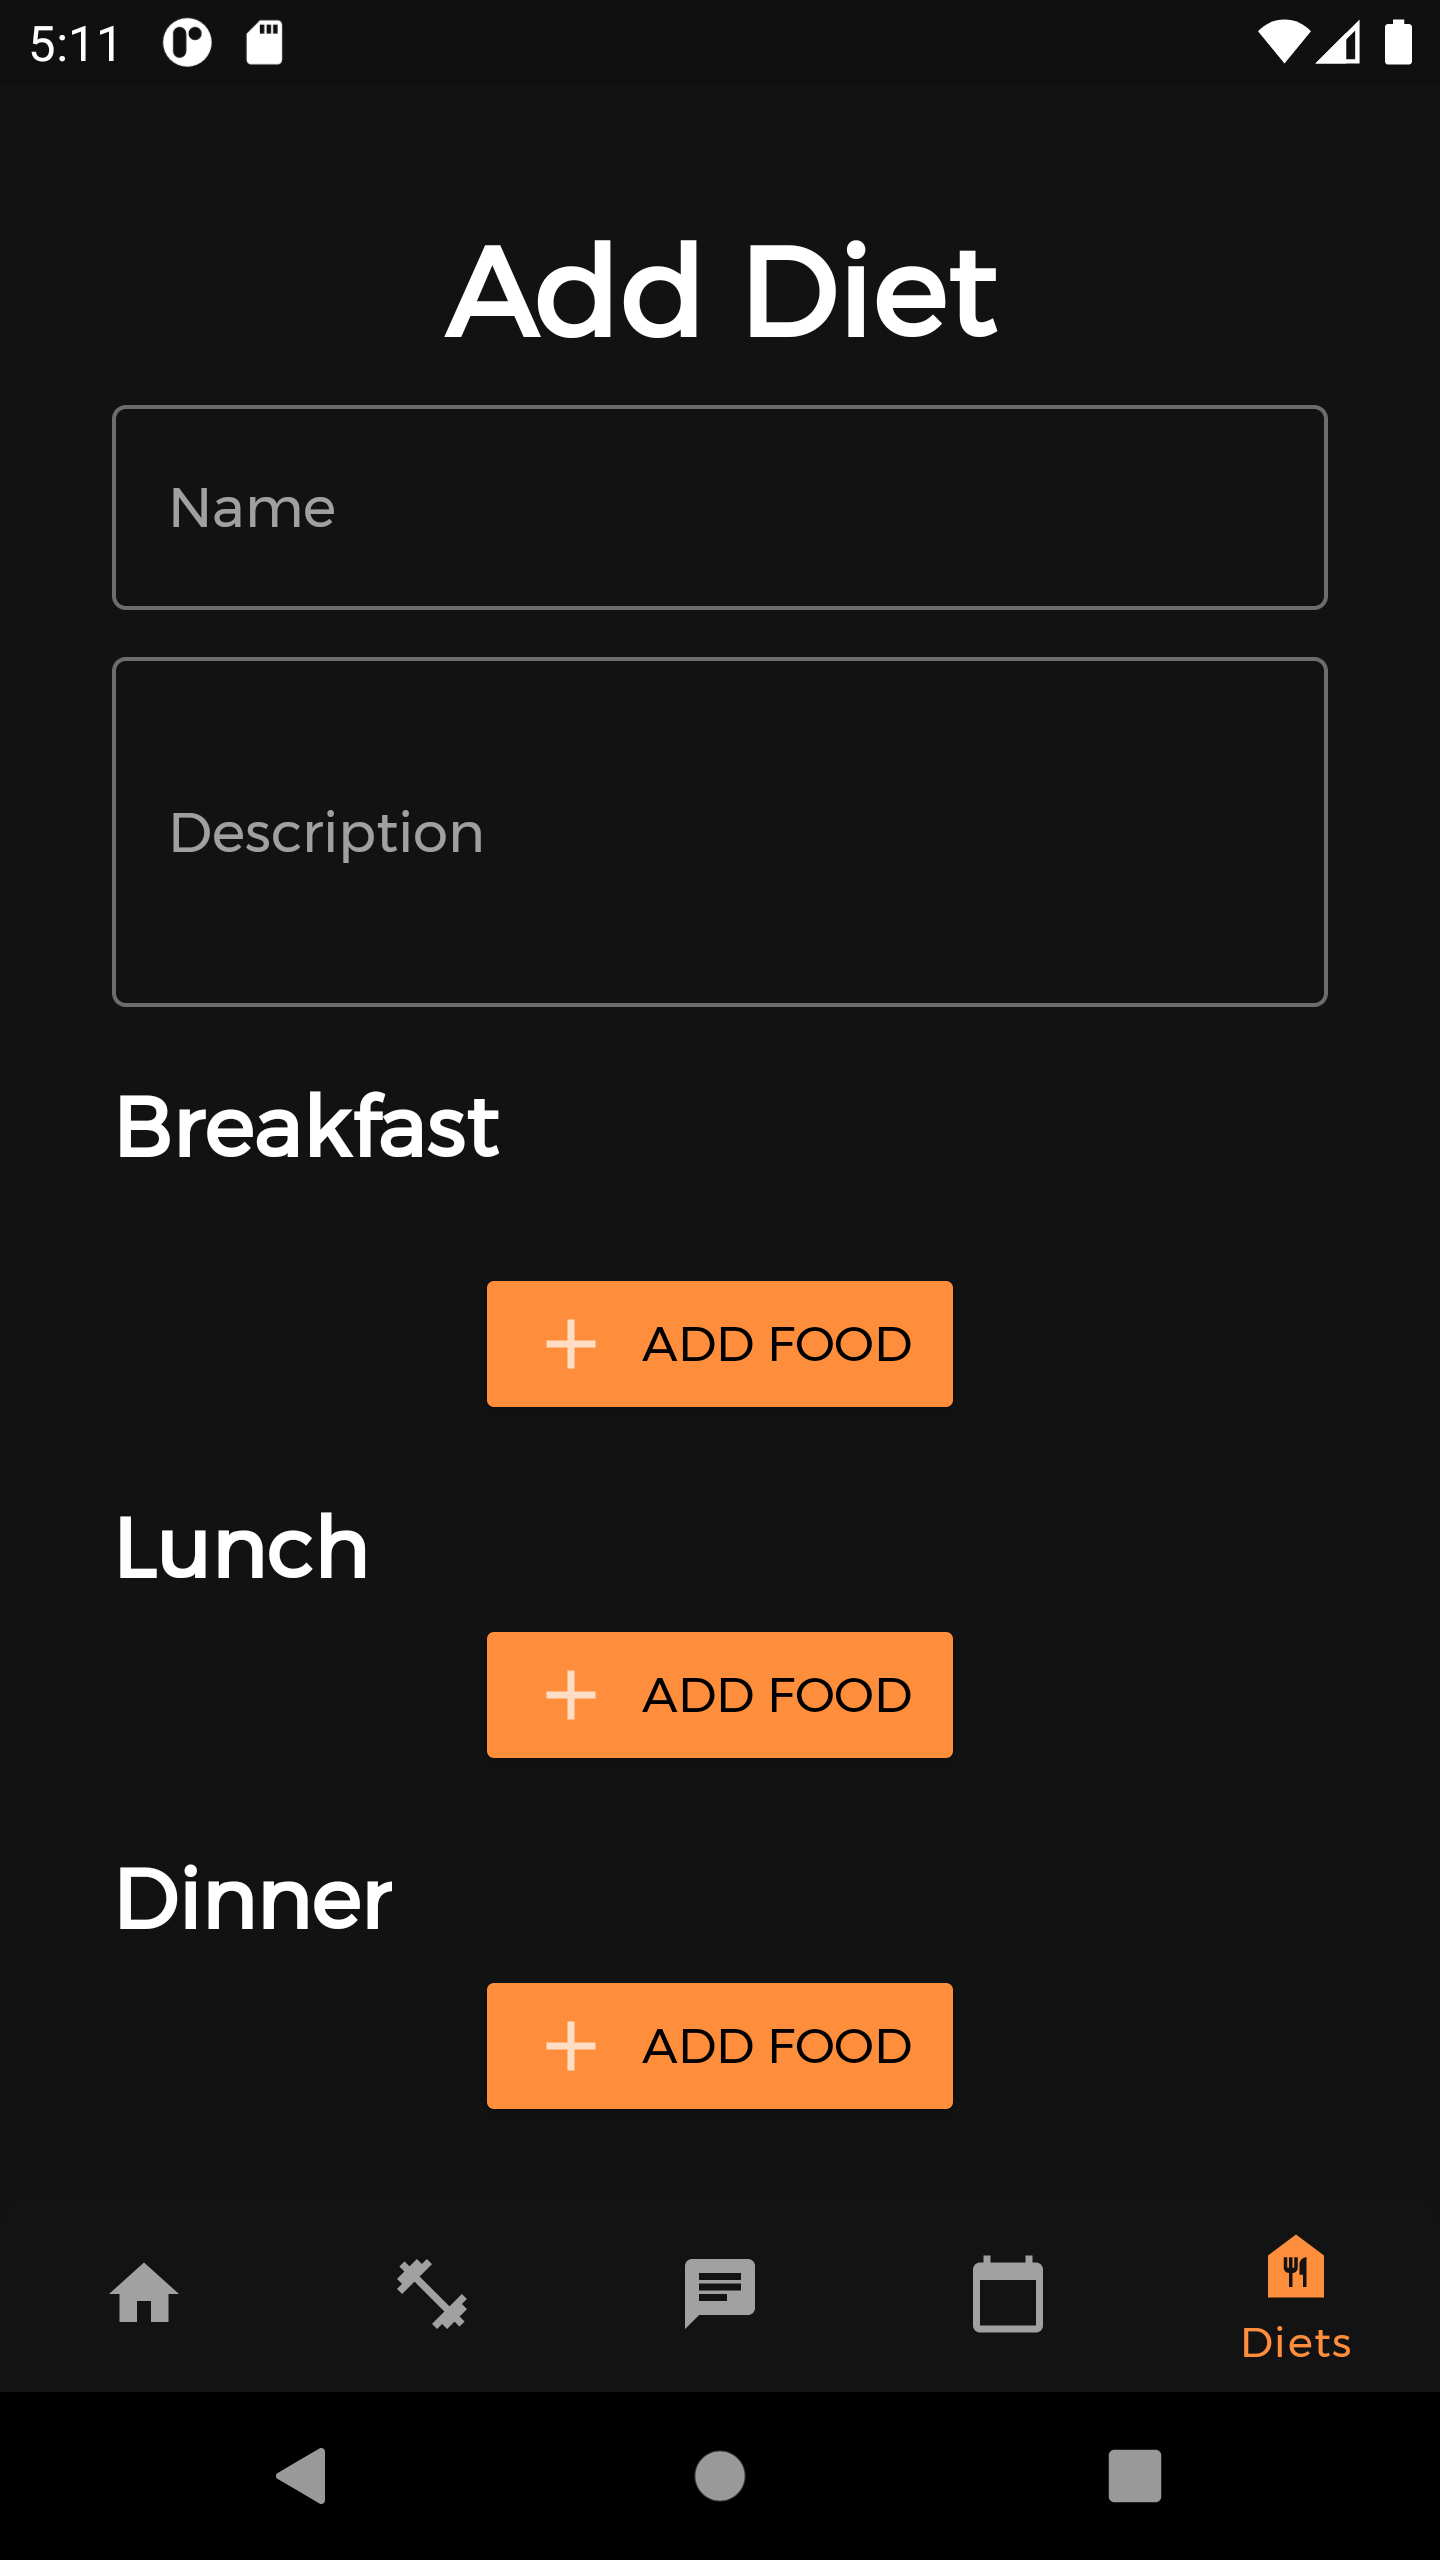
\includegraphics[width=\textwidth]{gymodo_add_diet}
\end{columns}

\end{frame}

\begin{frame}{Abstract}

\textbf{\color{gymodo_orange} Gyomodo} es una aplicación que tiene como objetivo resolver los problemas que puedan tener los gimnasios en estos tiempos modernos, pero sobre todo, problemas originados a partir de la pandemia del Covid-19.

\begin{itemize}
\item Reservar hora en el gimnasio
\item Crear workouts
\item Crear dietas, escaneando los productos
\item Ver noticias
\item Publicar posts con comentarios, una mini red social
\end{itemize}

\end{frame}

\end{document}